% Template for Cogsci submission with R Markdown

% Stuff changed from original Markdown PLOS Template
\documentclass[10pt, letterpaper]{article}

\usepackage{cogsci}
\usepackage{pslatex}
\usepackage{float}
\usepackage{caption}

% amsmath package, useful for mathematical formulas
\usepackage{amsmath}

% amssymb package, useful for mathematical symbols
\usepackage{amssymb}

% hyperref package, useful for hyperlinks
\usepackage{hyperref}

% graphicx package, useful for including eps and pdf graphics
% include graphics with the command \includegraphics
\usepackage{graphicx}

% Sweave(-like)
\usepackage{fancyvrb}
\DefineVerbatimEnvironment{Sinput}{Verbatim}{fontshape=sl}
\DefineVerbatimEnvironment{Soutput}{Verbatim}{}
\DefineVerbatimEnvironment{Scode}{Verbatim}{fontshape=sl}
\newenvironment{Schunk}{}{}
\DefineVerbatimEnvironment{Code}{Verbatim}{}
\DefineVerbatimEnvironment{CodeInput}{Verbatim}{fontshape=sl}
\DefineVerbatimEnvironment{CodeOutput}{Verbatim}{}
\newenvironment{CodeChunk}{}{}

% cite package, to clean up citations in the main text. Do not remove.
\usepackage{apacite}

% KM added 1/4/18 to allow control of blind submission


\usepackage{color}

% Use doublespacing - comment out for single spacing
%\usepackage{setspace}
%\doublespacing


% % Text layout
% \topmargin 0.0cm
% \oddsidemargin 0.5cm
% \evensidemargin 0.5cm
% \textwidth 16cm
% \textheight 21cm

\title{English Negative Constrctions and Communicative Functions in Early Child
Language}


\author{{\large \bf Morton Ann Gernsbacher (MAG@Macc.Wisc.Edu)} \\ Department of Psychology, 1202 W. Johnson Street \\ Madison, WI 53706 USA \AND {\large \bf Masoud Jasbi (jasbi@ucdavis.edu)} \\ Department of Linguistics, 469 Kerr Hall, One Shields Avenue \\ Davis, CA 95 USA}


\begin{document}

\maketitle

\begin{abstract}
How does negation emerge in early conceptual and linguistic development?
Previous research has hypothesized that negation develops to express
different communicative functions such as rejection, non-existence, or
prohibition. However, these functions have been challenging to detect
and classify by human annotators using contextual cues. Consequently, in
previous research we have been limited to relatively small number of
children and small samples of their speech. In this study, we consider
specific syntactic constructions as proxies for communicative functions
and examine their developmental trajectories in children's speech. We
used automatic annotation and identification of seven different
functions in a large corpus of child-parent interactions. Our analyses
demonstrated frequent usage of negation in all seven functions between
the ages of 24 - 36 months; yet there are notable differences in
production variability of negation depending on the specifc function
examined.

\textbf{Keywords:}
negation; acquisition; development, semantics, pragmatics, syntax, child
language.
\end{abstract}

\hypertarget{introduction}{%
\section{Introduction}\label{introduction}}

Negation is an abstract concept crucial to everyday communication. It
can help a coffee shop divide its menu into ``coffee'' and ``not
coffee'' sections, with the ``not coffee'' section bringing together
diverse items with no common label. It can inform us to regulate each
others' actions in a sign like ``no mask, no entry''. It can also
communicate our deepest wants and dislikes as in ``I don't like
Mondays''. But how does the abstract concept of negation emerge in the
human mind? What are the specific communicative functions that negation
combines with in early language development?

Starting a century and a half ago, Darwin (1872) thought that negation
has roots in the expression of human emotions and desires. He
hypothesized the earliest manifestation of negation and affirmation in
infants is when they refuse food from parents, by withdrawing their
heads laterally, or when they accept the food, by inclining their heads
forward. He suggested that head shaking and nodding as common gestures
for negation and affirmation have developed from this early habit.
Similarly, many researchers studying early functions of negative
morphemes like \emph{no} proposed that children use them to ``reject''
or ``refuse'' (Bloom, 1970; Choi, 1988; Pea, 1978). For example, when
they are asked ``do you want juice?'', they may say ``no'', ``not want
it'', or ``don't like it''. Pea (1978) proposed this negation function
is the first to emerge in children's early speech.

Bloom (1970) argued that the use of negation to expresses
``non-existence'' emerges before rejection or refusal. For example, when
an object that children expect to be present is not present, children
may say: ``no window'', ``no fish in the bathroom'', or ``I do not have
underpants''. Two close concepts to non-existence are ``disappearance''
and ``non-occurrence'' (Pea, 1978; Villiers \& Villiers, 1979).
Disappearance refers to situations where an object disappears and
children use negation to express it (e.g.~``no food. all gone'' or ``no
more noise''). Non-occurrence refers to cases when an expected action or
event does not occur as in ``not working'' or ``doggie not barking''.
Some researchers referred to these cases as ``failures'' and included
examples like ``no fit in da box'' or ``it don't fit''
(Cameron-Faulkner, Lieven, \& Theakston, 2007; Choi, 1988).
Non-existence can also be expressed by negation of locative
prepositional phrases (e.g.~``no in there'' or ``daddy was not on the
phone''). While rejection was hypothesized to interact with human
emotions and desires, non-existence (broadly construed to include
``disappearance'' and ``non-occurrence'') likely interacts with human
perception. Choi (1988) proposed that children's early linguistic
negation is used to express both rejection and non-existence.

Additionally, Choi (1988) introduced ``prohibition'' and suggested that
it emerges as early as rejection and non-existence. In cases of
prohibition, children use negation to stop others from performing
actions; for example ``don't go'' or ``do not spill milk''. A special
case of prohibition is ``self-prohibition''. For example, a child may
approach prohibited food but immediately say ``no, don't eat'' to stop
themselves. A function similar to prohibition is ``inability''
(e.g.~\emph{I can't reach} / \emph{I cannot zip it}), in that both
involve conceptualizing actions and negating them, possibly interacting
with early development of motor control. Choi (1988) suggested that
expression of inability emerges after the first phase, namely
non-existence, rejection, and prohibition.

``Denial'' is another function of negation that is argued to be late in
development. Bloom (1970) defined it as asserting that ``an actual or
supposed predication was not the case'', for example ``It's not sharp''.
Later researchers formulated it as ``truth-functional negation'' because
it is used to negate the truth of a proposition (Cameron-Faulkner et
al., 2007; Pea, 1978). However, this definition depends on the assumed
logical system and its assumptions on what type of propositions receive
truth values. A particular sub-function of denial is ``labeling'', which
is realized as the negation of nominal or adjectival predicates such as
``this is not a bunny'' or ``not red''. These utterances are often used
to introduce new linguistic labels by parents and in turn may facilitate
word learning (Clark, 2010). Conversely, labeling and word learning may
aid the development of abstract negation.

Despite considerable research on early functions of negation, their
developmental trajectories in children's productions have remained
unclear. Different studies have claimed different order of acquisition
(Pea, 1978). In a recent study, Nordmeyer \& Frank (2018) looked at the
speech of five children in the Providence corpus (Demuth, Culbertson, \&
Alter, 2006) and found a great deal of individual differences in how
early a negative function is attested. This is partly because previous
studies have had to rely on human annotation and identification of
functions from corpus data, a time-consuming and difficult process that
has limited previous studies to a handful of children and a relatively
small sample of their speech.

Our study addresses this issue by using syntactic constructions as a
proxy for communicative functions. We used a large collection of child
language corpora (MacWhinney, 2000) with part of speech tags and
syntactic dependency relations. We automatically selected constructions
that conveyed the functions discussed in prior research and asked: (1)
how early do these constructions emerge in children's speech and what's
their trajectory? (2) within the same communicative function, does the
developmental trajectory differ depending on particular lexical items
that negation modifies (e.g.~\emph{like} or \emph{want} for rejection)?
(3) taking all functions into account, do they share similar
developmental characteristics, or would there be function-specific
differences?

\begin{table*}[h]
\small
\centering
\begin{tabular}{rrr}
  \hline
 \textbf{Function} & \textbf{Linguistic Composition} & \textbf{Examples} \\
  \hline
Rejection & with \textit{like} or \textit{want} & \textit{I not like it}, \textit{not want it}  \\
Non-existence & expletives; with a nominal; \textit{no more} & \textit{there is no soup}; \textit{no juice}; \textit{no more milk} \\
Prohibition & with imperative subjectless \textit{do} & \textit{do not spill milk} \\
Inability & with modal \textit{can} & \textit{I cannot zip it} \\
Labeling & modifying nominal or adjectival predicatives & \textit{that's not a crocodile}; \textit{it's no interesting} \\
Epistemic negation & with \textit{know}, \textit{think}, \textit{remember}  & \textit{I not know} \\
Possession & with \textit{have}; or possesive pronouns & \textit{not have the toy}; \textit{not mine} \\
   \hline
\end{tabular}
\caption{Communicative functions of negation in early child language of English.}
\end{table*}

\hypertarget{experiments}{%
\section{Experiments}\label{experiments}}

\hypertarget{data-and-preprocessing}{%
\subsection{Data and preprocessing}\label{data-and-preprocessing}}

For developmental data of child language in English, we turned to the
CHILDES database (MacWhinney,
2000).\footnote{Code and data are in quarantine at https://somewhereonearth.}.
We focused on speech produced by children with typical development
within the age range of 12 - 72 months. Negative structures were first
identified based on whether a structure contains any of the three
negative morphemes: \emph{no}, \emph{not} and \emph{n't}. Since the
matters of interest are individual utterances and what negation
\emph{combines} with, cases consisting of one negative morpheme were
excluded (e.g.~\emph{no}!). Preprocessing led to a data set of 365,260
negative utterances from a total of 811 children across 56 corpora.

\hypertarget{negation-functions}{%
\subsection{Negation functions}\label{negation-functions}}

Besides the communicative function of rejection, non-existence,
prohibition, inability and denial (labeling), we expanded with two other
functions: epistemic negation (Choi, 1988) and possession (see Table 1).
For each function, we first characterized the syntactic features of the
linguistic structures that the negative morphemes are combined with.
Then negative utterances of different communicative functions were
automatically extracted in a rule-based fashion, i.e.~based on the
syntactic characteristics. In order to do this, we resorted to the
available morphosyntactic information provided from CHILDES (Sagae,
Davis, Lavie, MacWhinney, \& Wintner, 2010), such as part-of-speech
(POS) tags as well as grammatical or syntactic dependency relations.
After extracting negative utterances, the developmental trajectories of
different constructions of interest were analyzed.

In what follows we introduce each construction and present the results.
While our focus is child utterances, we used parents' speech as
references and therefore our plots often contrast the relative frequency
(or ratio) of these constructions between children's and parents'
production at the corresponding age of the child.

\hypertarget{rejection}{%
\subsubsection{Rejection}\label{rejection}}

For the function of rejection, we examined cases where the lemma of the
head verb of the phrase is either \emph{like} or \emph{want}, and the
head verb is modified by one of the three negative morphemes. Each of
the utterances either takes a subject or has no subject at all. And the
existence of a subject was determined via searching for a word in the
utterance that has the \emph{SUBJ} dependency relation with the head
verb.

Additionally, other than expressions that the speaker used to describe
their own emotion (e.g.~(1)) or their (in)ability to do so (e.g.~(2)),
we also included cases that express rhetorical inquiries of emotions
from one interlocutor addressed to another (e.g.~(3)) as well as
instances where the speaker is describing the emotion of somebody else
(e.g.~(4)). Overall our data extraction resulted in a total of 21,034
utterances (Child: 9,608; Parent: 11,426).

~ (1) \emph{I no like sea} / \emph{don't wanna go}

~ (2) \emph{I can't like that}

~ (3) \emph{don't you wanna try it}

~ (4) \emph{Sarah doesn't like that either}

To compare the patterns between child and parent speech, we measured the
following four metrics. The first one is the relative ratio of each of
the three negative morphemes overall. For instance, given the 9,608
utterances from child speech that serve as rejections, there are 8,531
cases with the negative morpheme \emph{no}; then the ratio of these
utterances was calculated as 8,531 / 9,608 = 0.41. The second one is the
relative ratio of negative morphemes within different head verbs
(e.g.~\emph{like} vs.~\emph{want} for rejection). For example, again
with child speech that express rejections, utterances where the negative
morphemes modify the head verb \emph{like} occur for 3,268 times; then
the ratio of these cases was computed as 3,268 / 9,608 = 0.16. The third
one is the relative ratio of the negative utterances at different ages
of the child. For instance, for rejection, at the age of 36 months, the
total number of instances with the negative morphemes in child speech is
888; then their ratio was calculated as 888 / 9,608 = 0.04.

The last one is the amount of variability in the production of the
specific function across the age span of the child, which was measured
with entropy (Cover \& Thomas, 1991). For example, after computing the
relative ratio \emph{P(x\_i)} of the negative utterances at a number of
\(N\) ages of the child for the specific function, the production
variability is calculated using the equation below. \begin{equation}
H(X) = -\sum_{i=1}^N P(x_i)log_2P(x_i) 
\end{equation}

\begin{CodeChunk}
\begin{figure}[H]

{\centering 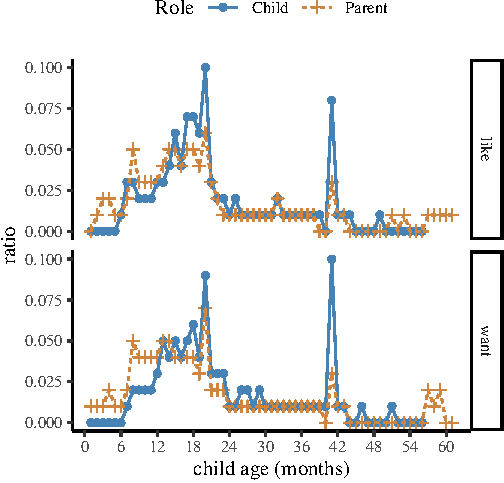
\includegraphics{figs/emotion-1} 

}

\caption[Rejection]{Rejection}\label{fig:emotion}
\end{figure}
\end{CodeChunk}

In both child and parent speech, when articulating desires or emotions
with either of the two head verbs \emph{like} and \emph{want}, the most
frequently used negative morpheme is \emph{n't} combined with an
auxiliary verb. Comparing the two different head verbs, overall the
negative morphemes co-occur with \emph{want} more frequently. With that
being said, the amount of variability in both child and parent
production is similar, a pattern that holds for both head verbs (Child
\emph{like}: 0.12; Child \emph{want} 0.12; Parent \emph{like}: 0.12;
Parent \emph{want}: 0.12).

On the other hand, when looking at the developmental trajectory, as
presented in Figure 1, children's usage of negative morphemes is
comparable regardless of the particular head verb. In general, children
start applying the negative morphemes for the function of rejection more
regularly around the age of 22 months. Within the context of the corpus
data that we analyzed, their usage of these morphemes is the most
frequent during the age range of 25 - 36 months.

\hypertarget{non-existence}{%
\subsubsection{Non-existence}\label{non-existence}}

For the function of non-existence, we extracted utterances that either
have expletives marked by \emph{there} (e.g.~(5)), or cases where the
negative morphemes are modifying a nominal (i.e.~its syntactic head
based on the CHILDES annotation is a nominal; e.g.~(6)). With utterances
such as (6) in particular, in order to not confuse with the function of
labeling (see below), we did not include any cases where the syntactic
head of the negative morphemes is a predicate of a copula verb
(e.g.~\emph{this is not candy}). This led to a total of 34,672
utterances (Child: 16,866; Parent: 17,806).

~ (5) \emph{there's no water}

~ (6) \emph{no (more) candy} / \emph{not your mouth}

In both child and parent speech, the most frequently occurred negative
morphemes to indicate non-existence is \emph{no}. The amount of
production variability approximates 0.12 regardless of the specific
speaker. As shown in Figure 2, children began increasing their use of
the negative morphemes to express non-existence around the age of 22
months, which is similar to that for the function of rejection and in
opposition to what was initially proposed by Bloom (1970).

\begin{CodeChunk}
\begin{figure}[H]

{\centering 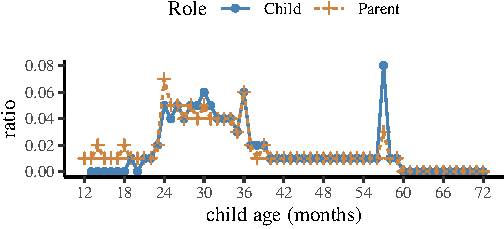
\includegraphics{figs/existence-1} 

}

\caption[Non-existence]{Non-existence}\label{fig:existence}
\end{figure}
\end{CodeChunk}

\hypertarget{prohibition}{%
\subsubsection{Prohibition}\label{prohibition}}

For utterances that articulate the function of prohibition, we focused
on cases where the negative morphemes are combined with the auxiliary
verb \emph{do} (\emph{do}, \emph{does}, \emph{did}) and the auxiliary
does not take any subject (e.g.~(7)). In certain cases the negative
morphemes and the auxiliary together modifies a head verb. For instances
as such, in order to not overlap with rejection, non-existence and
epistemic negation and possession (see below), our search excluded cases
where the head verb has any of the following lemma forms: \emph{like},
\emph{want}, \emph{know}, \emph{think}, \emph{remember}, \emph{have}.
This resulted in a total of 21,197 utterances (Child: 6,140; Parent:
15,057).

After applying our metrics, overall the most frequently used negative
morpheme is \emph{n't} when articulating prohibition. The amount of
production variability for this function is comparable in both child and
parent speech, with an approximate value of 0.12. Based on Figure 3,
children started more regular usage of negative morphemes to articulate
prohibition around the age of 23 months. This finding also corresponds
to the proposal from (Choi, 1988), which suggested that prohibition
emerges around similar times compared to rejection and non-existence.

~ (7) \emph{don't blame Charlotte} / \emph{don't}

\begin{CodeChunk}
\begin{figure}[H]

{\centering 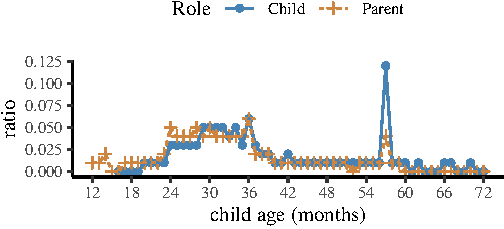
\includegraphics{figs/prohibition-1} 

}

\caption[Prohibition]{Prohibition}\label{fig:prohibition}
\end{figure}
\end{CodeChunk}

\begin{CodeChunk}
\begin{figure}[H]

{\centering 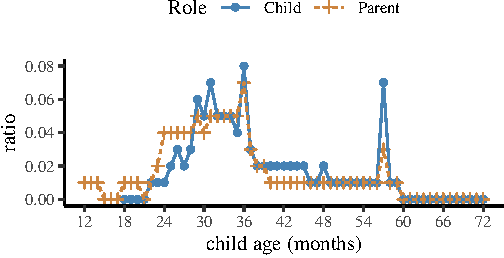
\includegraphics{figs/inability-1} 

}

\caption[Inability]{Inability}\label{fig:inability}
\end{figure}
\end{CodeChunk}

\hypertarget{inability}{%
\subsubsection{Inability}\label{inability}}

We analyzed instances where the negative morphemes co-occur with the
auxiliary \emph{can} (\emph{can} and \emph{could}; e.g.~(8)) for the
function of inability. Again, for instances with a head verb modified by
the negative morphemes and the auxiliary, we filtered out cases where
the head verbs are the focus for other functions. Cases that do not have
a subject (e.g.~\emph{can't play}) or do not contain a subject other
than I (e.g.~\emph{you can't do that}) could yield ambiguous readings
without taking a larger discourse context into account; they could be a
rhetorical question or also express the concept of prohibition.
Therefore to avoid potential ambiguity, we restricted our analyses only
to cases with a subject \emph{I}. This led to a subset of 9,150
utterances (Child: 5,410; Parent: 3,740).

~ (8) \emph{I can't see} / \emph{I can't}

Comparing child and parent production, the negative morpheme that is
used most frequently is also \emph{n't}. As shown in Figure 4, the
developmental trajectory of this function is similar to that for
prohibition (Choi, 1988), and the negative morphemes are applied more
regularly starting around the age of 23 months. The amount of production
variability in both child and parent speech is approximately 0.12.

\hypertarget{labeling}{%
\subsubsection{Labeling}\label{labeling}}

To capture the function of denials, in parituclar the instances of
labeling, we concentrated on cases where negative morphemes are adopted
to indicate the identity (e.g.~(9)), and/or characteristics (e.g.~(10))
of a predicative nominal. In addition, we also included instances where
the negative morphemes are used to modify a predicative adjective
(e.g.~(11)). Following these criteria, utterances where the negative
morpheme is modifying a nominal or adjectival predicate of a copula verb
were extracted. None of the utterances contained expletives (\emph{there
is no book}). The existence of a predicate was identified with the help
of POS information and dependency relation. The POS of the predicate has
to be either noun (\emph{n}) or adjective (\emph{adj}), and its
dependency relation with the copula has to be \emph{PRED}. This resulted
in a total of 20,329 utterances (Child: 4,793; Parent: 15,536).

~ (9) \emph{that's not a farmer}

~ (10) \emph{I'm not a heavy baby Mum}

~ (11) \emph{It's no good}

Comparing the three negative morphemes, the most frequently used is
\emph{not} regardless of the specific speaker, and the amount of
production variability is comparable (\textasciitilde0.12) between child
and parent speech. Based on results from Figure 5, the developmental
trajectory of using the negative morphemes in the domain of language
learning is comparable to previous domains. Children started using the
negative morphemes for the function of labeling more frequently around
the age of 24 months.

\begin{CodeChunk}
\begin{figure}[H]

{\centering 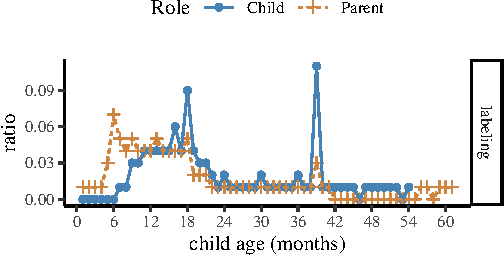
\includegraphics{figs/learning-1} 

}

\caption[Language learning via labeling]{Language learning via labeling}\label{fig:learning}
\end{figure}
\end{CodeChunk}

\hypertarget{epistemic-negation}{%
\subsubsection{Epistemic Negation}\label{epistemic-negation}}

The function of epistemic negation was originally discussed by Choi
(1988). Although there has been no proposal for negation originating in
children's understanding of their own or others' epistemic/mental
states, previous studies have reported many instances where the negative
morphemes are combined with mental state verbs such as \emph{know},
\emph{think}, and \emph{remember}. Here we focused on these three verbs
and analyzed utterances that articulate the concept of unknowing
(e.g.~(12)) or uncertainty (e.g.~(13)). The verbs in these cases are
modified by the negative morphemes or the combination of negation with
auxiliaries. By these search criteria, instances where the speaker
inquires about or describes the negative epistemic state of another
speaker (e.g.~(14)) were also selected. This led to a subset of 32,793
utterances in total (Child: 10,389; Parent: 22,404).

~ (12) \emph{I not know} / \emph{I didn't remember}

~ (13) \emph{I don't think so}

~ (14) \emph{don't you remember} / \emph{She doesn't know this}

\begin{CodeChunk}
\begin{figure}[H]

{\centering 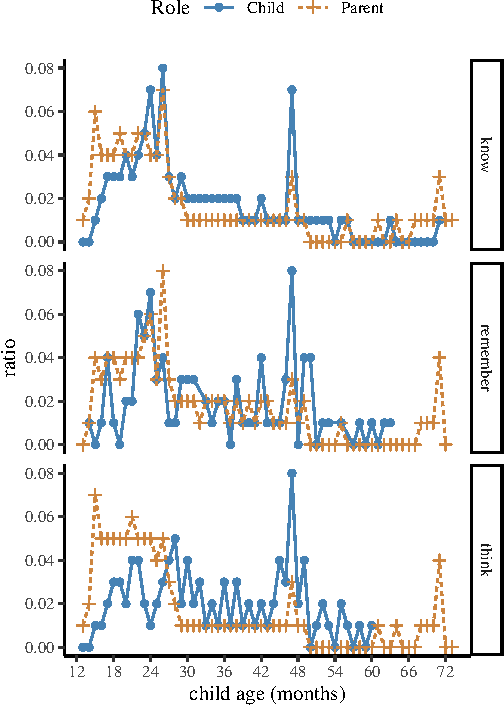
\includegraphics{figs/epistemic-1} 

}

\caption[Epistemic]{Epistemic}\label{fig:epistemic}
\end{figure}
\end{CodeChunk}

In both child and parent speech, the most frequently used negative
morpheme that modifies epistemic state is \emph{n't}, a pattern that is
consistent across the three different head verbs. And the negative
morphemes tend to co-occur more often in cases that describe the state
of unknowing, which is indicated mainly by the verb \emph{know}. Based
on results from Figure 6, the production of \emph{know} for expressions
of epistemic state starts earlier in comparison to \emph{remember} and
\emph{think}. On the other hand, the production variability for each of
the head verb (\textasciitilde0.12) is comparable to each other
regardless of the particular speaker. Overall, children began to apply
the negative morphemes to articulate this function in a more regular
fashion around the age of 25 months.

\hypertarget{possession}{%
\subsubsection{Possession}\label{possession}}

The last function that we investigated includes utterances that are
combined with negative morphemes to denote possession. Specifically, we
selected cases where the negative morphemes are modifying a possessive
pronoun (e.g.~(15)), as well as instances where the negative morphemes
are combined with auxiliary verbs to modify a head verb with the lemma
form \emph{have} (e.g.~(16)). Again similarly to our search for
utterances that express non-existence, we excluded cases in which the
syntactic head of the negative morphemes is a predicate of a copula verb
(e.g.~\emph{this is not mine}). The number of utterances that were
subjected to analysis for this function is 9,265 (Child: 2,899; Parent:
6,366). The developmental trajectory for this function, as shown in
Figure 7, is comparable to the other functions, where children started
to combine negative morphemes around the age of 22 months.

~ (15) \emph{not mine}

~ (16) \emph{I don't have it}

\begin{CodeChunk}
\begin{figure}[H]

{\centering 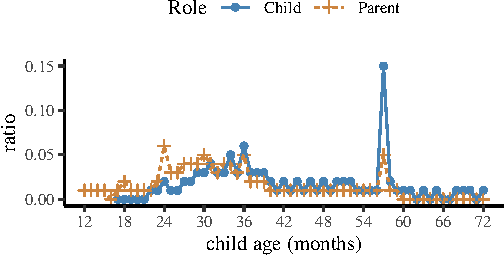
\includegraphics{figs/possession-1} 

}

\caption[Possession]{Possession}\label{fig:possession}
\end{figure}
\end{CodeChunk}

\hypertarget{overall}{%
\subsubsection{Overall}\label{overall}}

\begin{figure*}[h]
\begin{CodeChunk}


\begin{center}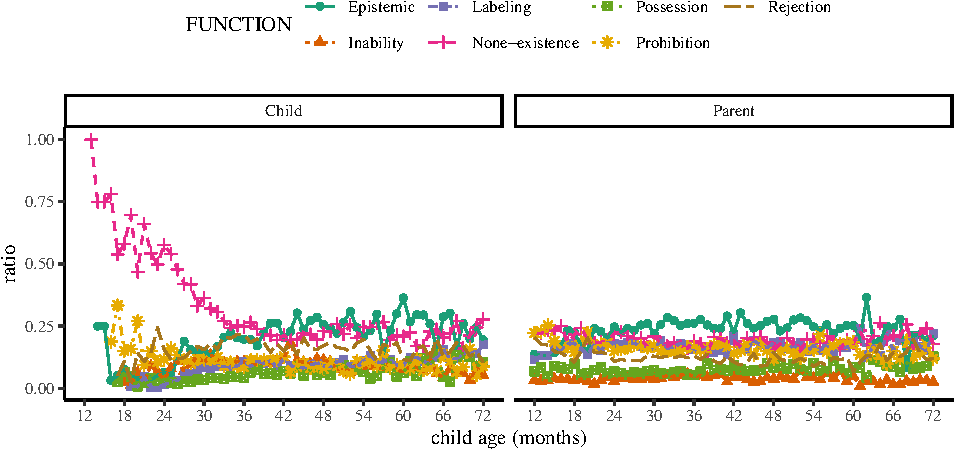
\includegraphics{figs/all-1} \end{center}

\end{CodeChunk}
\caption[This image spans both columns]{All functions.}\label{fig:all}
\end{figure*}

Figure 8 shows the developmental trajectory for all analyzed negative
functions. The y-axis is the relative frequency of each construction
relative to the frequency of all constructions within a monthly age
period. Children's negative utterances bear considerable resemblance to
parent speech in terms of the overall production frequency. Early on,
the most frequently applied function is non-existence, while the
functions with relatively smaller number of occurrences include
possession and inability. There are a number of observable differences
with respects to the production variability of individual functions.
Comparing across functions, the usage of negative morphemes for
non-existence is the most variable, with considerable variability in
child speech (Child: 1.61; Parent: 1.08). The opposite pattern is
observed for prohibitions (Child: 0.62; Parent: 0.92) and labeling
(Child: 0.49; Parent: 0.94).

\hypertarget{discussion}{%
\section{Discussion}\label{discussion}}

In this study, we used automatic and large-scale annotation and analysis
of negative constructions in children's and parents' speech using POS
tags and syntactic dependency relations. We presented analyses negative
utterances that convey rejection, non-existence, prohibition, inability,
labeling, epistemic states and possession. Overall our results show that
negation is frequently used in constructions that convey these functions
between the ages of 24 to 36 months.

It is important to note that similar to prior studies, our conclusions
are limited to children's production. While it is possible that patterns
in children's production reflect their comprehension and semantic
development overall, this is not guaranteed. Most importantly, there are
production-specific effects (e.g.~length of utterance, ease of
pronunciation) that we have not taken into account yet. Thus, results
presented here cannot support a specific order of acquisition
hypothesis. We plan to take production-specific factors into account in
the future. More importantly, experiments testing children's
comprehension of negative utterances that serve different communicative
functions are necessary in order to understand the origin of negation
more thoroughly.

In future work, we plan to investigate the production trajectory of
positive counterparts to our negative structures (e.g.~\emph{I know} for
\emph{I don't know}). This would allow us to compare the production of
positive and negative constructions and control for the production
trajectory of specific constructions regardless of whether negation is
present. We also intend to focus on individual differences among
children given our methods and analyses. Lastly, our experiments thus
far have concentrated on multi-word syntactic structures at the
utterance level, therefore cases where negations are used as discourse
markers in single-word or few-word expressions were excluded. However,
discourse markers as responses to previous utterances have important
semantic and conceptual roles in the communication between children and
parents (e.g.~Parent: \emph{do you want some bread?}; Child: \emph{no no
no}). Inclusions of negative structures at the discourse level would
allow us to paint a more clear picture about the development of
negation.

\hypertarget{references}{%
\section{References}\label{references}}

\setlength{\parindent}{-0.1in} 
\setlength{\leftskip}{0.125in}

\noindent

\hypertarget{refs}{}
\leavevmode\hypertarget{ref-bloom1970language}{}%
Bloom, L. M. (1970). \emph{Language development: Form and function in
emerging grammars} (PhD thesis). Columbia University.

\leavevmode\hypertarget{ref-cameron2007part}{}%
Cameron-Faulkner, T., Lieven, E., \& Theakston, A. (2007). What part of
no do children not understand? A usage-based account of multiword
negation. \emph{Journal of Child Language}, \emph{34}(2), 251.

\leavevmode\hypertarget{ref-choi1988semantic}{}%
Choi, S. (1988). The semantic development of negation: A
cross-linguistic longitudinal study. \emph{Journal of Child Language},
\emph{15}(3), 517--531.

\leavevmode\hypertarget{ref-clark2010adult}{}%
Clark, E. V. (2010). Adult offer, word-class, and child uptake in early
lexical acquisition. \emph{First Language}, \emph{30}(3-4), 250--269.

\leavevmode\hypertarget{ref-cover_elements_1991}{}%
Cover, T. M., \& Thomas, J. A. (1991). \emph{Elements of information
theory}. New York: Wiley.

\leavevmode\hypertarget{ref-darwin1872expression}{}%
Darwin, C. (1872). \emph{The expression of the emotions in man and
animals}. John Murray.

\leavevmode\hypertarget{ref-demuth2006word}{}%
Demuth, K., Culbertson, J., \& Alter, J. (2006). Word-minimality,
epenthesis and coda licensing in the early acquisition of English.
\emph{Language and Speech}, \emph{49}(2), 137--173.

\leavevmode\hypertarget{ref-macwhinney2000childes}{}%
MacWhinney, B. (2000). \emph{The childes project: Tools for analyzing
talk. Transcription format and programs} (Vol. 1). Psychology Press.

\leavevmode\hypertarget{ref-nordmeyer2018individual}{}%
Nordmeyer, A., \& Frank, M. C. (2018). Individual variation in
children's early production of negation. In \emph{CogSci}.

\leavevmode\hypertarget{ref-pea1978}{}%
Pea, R. (1978). \emph{The development of negation in early child
language} (PhD thesis). University of Oxford.

\leavevmode\hypertarget{ref-sagae2010morphosyntactic}{}%
Sagae, K., Davis, E., Lavie, A., MacWhinney, B., \& Wintner, S. (2010).
Morphosyntactic annotation of childes transcripts. \emph{Journal of
Child Language}, \emph{37}(3), 705--729.

\leavevmode\hypertarget{ref-de1979form}{}%
Villiers, P. A. de, \& Villiers, J. G. de. (1979). Form and function in
the development of sentence negation. \emph{Papers and Reports on Child
Language Development}, \emph{17}, 57--64.

\bibliographystyle{apacite}


\end{document}
